
% -----------------------------------------------------------------------------------------------------------------
%\newpage
%\thispagestyle{empty}
%\rule{\linewidth}{2pt}
\chapter{Análisis dinámico de la familia de Homeier Generalizado}\label{capitulodinamica}
En este capítulo vamos a estudiar el comportamiento dinámico de la familia de métodos iterativos diseñada en la la Sección \ref{seccionHG}, sobre polinomios cuadráticos. Este estudio nos va a permitir elegir los elementos de la familia con mejor estabilidad y determinar cuáles no deben ser usados por sus malas propiedades numéricas.

La aplicación de métodos iterativos en polinomios da lugar a funciones racionales cuya dinámica compleja no es del todo conocida, excepto en el caso del método de Newton (ver, por ejemplo, \cite{blanchard}). Desde el punto de vista numérico, el comportamiento dinámico de la función racional asociada a un método iterativo nos da información importante sobre su estabilidad y fiabilidad. En este sentido, Varona en \cite{Va} y Amat et al. en \cite{Amat3} describieron el comportamiento dinámico de muchas familias bien conocidas de métodos iterativos. Más recientemente, en \cite{ABBP,CCT,CGTVV,CTV,GHR,NCS,SNC}, los autores analizan, bajo el punto de vista de la dinámica compleja, el comportamiento cualitativo de diferentes métodos iterativos conocidos o familias, como las de King, Chebyshev-Halley o la c-familia. 

Cuando se realiza este tipo de análisis aparecen distintos comportamientos numéricos patológicos,
como órbitas periódicas, puntos fijos atractores distintos de la solución del problema, etc. Una herramienta muy útil para entender el comportamiento de los
diferentes miembros de la familia de métodos es el plano de parámetros, que nos ayuda a seleccionar los miembros más estables de la familia. 

Bajo el punto de vista de la dinámica compleja, estudiaremos la convergencia general de la familia (\ref{generalizacion}) en polinomios cuadráticos. Se sabe que las funciones racionales asociadas a los miembros de la familia que actúan sobre un polinomio pueden ser
transformadas por una aplicación afín sin cambios cualitativos en la
dinámica de la familia.

Primero se analizan los puntos fijos de la función racional asociada a la familia, se estudia su estabilidad y posteriormente se calculan los puntos críticos libres. Para ello, usaremos el software descrito en \cite{CCT}.

Cabe destacar que estos resultados, junto con los obtenidos en la Sección \ref{seccionHG}, han sido enviados a la revista \textit{``Nonlinear Dynamics''}, bajo el título \textit{``Chaos and Convergence of a family generalizing Homeier's method with damping parameters''}, y están, actualmente, pendientes de publicación.

\begin{theorem}[Teorema del escalado]
	Sea $A(z)=a z+ b$ una transformación afín en $\mathbb{C}$.
	Sea también $f(x)$ una función real y $g(z)=\lambda(f\circ
	A)(z)$. Entonces, los operadores asociados a la familia \eqref{generalizacion}
	$T_f$ y $T_g$ son conjugados afinamente por $A$. Eso es, $\left(A\circ
	N_g\circ A^{-1}\right)(z)=N_f(z)$, para todo $z \in \mathbb{C}$.
\end{theorem}

\begin{proof} Demostraremos la igualdad equivalente:
	\[
	\left(A\circ T_g \right)(z)=\left(T_f\circ A\right)(z), \forall z \in \mathbb{C}.
	\]
	Desarrollando la parte de la derecha,
	\begin{eqnarray*}
		\left(T_f\circ A\right)(z)&=&T_f(A(z))\\
		&=& A(z)-\left[ \gamma \frac{f(A(z))}{f'\left(A(z)-\frac{1}{2\gamma}\frac{f(A(z))}{f'(A(z))}  \right)}+(1-\gamma)\frac{f(A(z))}{f'(A(z))}\right].
	\end{eqnarray*}
	Por otro lado, usando que $A(u-v)=A(u)-A(v)+b$ y que $A(c u)=c a u +b$, se puede comprobar que
	\begin{equation*}
	\left(A\circ T_g \right)(z)=a T_g(z)+b=\left(T_f\circ A\right)(z)
	\end{equation*}
	y el teorema queda demostrado. $\Box$
\end{proof}

\begin{theorem}
	Sea $g(z)=a_1 z^2+a_2 z+a_3$, $a_1\neq 0$, un polinomio cuadrático con raíces simples. Entonces, $g(z)$ puede reducirse a $p(z)=z^2+c$, mediante una transformación afín donde $c=4a_1a_3-a_2^2$. Esta aplicación afín induce una conjugación en $R_g(z)$ y $R_p(z)$.
\end{theorem}

Entonces, podemos usar el polinomio cuadrático arbitrario
$p(z)=(z-a)(z-b)$. Para $p(z)$, el operador de la familia es la función racional:
\begin{equation}
T_{p}(z,\gamma,a,b)=\frac{(\gamma -1) (a-z) (z-b)}{a+b-2 z}+\frac{\gamma  (z-a) (z-b)}{-2 \left(\frac{(a-z) (b-z)}{2 \gamma  (a+b-2 z)}+z\right)+a+b}+z
\end{equation}
que depende de los parámetros $\gamma$, $a$ y $b$.

Blanchard en \cite{blanchard} consideró la conjugación de plano
$\displaystyle h\left( z\right) =\frac{z-a}{z-b}$, (transformación de M\"{o}bius) con las siguientes propiedades:
\begin{equation*}
\mbox{i)} \ \  h\left( \infty \right) =1, \ \  \ \ \mbox{ii)} \ \  h\left(a\right) =0, \ \  \ \ \mbox{iii)} \ \  h\left( b\right) =\infty ,
\end{equation*}
y demostró que, para polinomios cuadráticos, el operador de Newton es conjugado al plano racional $z^{2}$. De forma análoga, el operador $T_{p}(z,\gamma,a,b)$ en polinomios cuadráticos es conjugado al operador $O_{p}\left( z,\gamma\right)$,
\begin{equation}\label{operadorking}
O_{p}\left(z,\gamma\right)=\left( h \circ T_{p} \circ h^{-1} \right) \left( z\right)=\frac{z^3 (\gamma  (z+2)-1)}{\gamma +(2 \gamma -1) z}
\end{equation}
Observemos que los parámetros $a$ y $b$ han desaparecido en $O_{p}(z,\gamma)$, con lo que el operador depende únicamente del parámetro de la familia.

%%%%%%%%%%%%%%%%%%%%%%%%%%%%%%%%%%%%%%%%%%%%%%%%%%%%%%%
\section{Análisis de los puntos fijos y críticos}
Los puntos fijos de $O_{p}\left( z,\gamma\right)$ son las raíces de la ecuación $O_{p}\left( z,\gamma\right)=z$, que son, $z=0$, $z=\infty$ (asociados a las raíces $a$ y $b$ de $p(z)$ previas a la transformación de M\"{o}bius)
y, para $\gamma \neq 0$, los siguientes puntos fijos extraños
\begin{itemize}
	\item $s_1(\gamma)=1$,
	\item $s_2(\gamma)=\frac{1}{2 \gamma }(-\sqrt{5 \gamma ^2-6 \gamma +1}-3 \gamma +1)$,
	\item $s_3(\gamma)=\frac{1}{2 \gamma }(\sqrt{5 \gamma ^2-6 \gamma +1}-3 \gamma +1)$.
\end{itemize}

En el siguiente resultado describimos algunas relaciones entre los puntos fijos extraños
\begin{lemma} El número de puntos fijos extraños simples del operador $O_{p}\left( z,\gamma\right)$ es tres, excepto en los casos:
	\begin{itemize}
		\item[i)] Si $\gamma=1$, entonces la expresión del operador es $O_{p}(z,1)=z^3$, por lo que el único punto fijo extraño es $z=1$.
		\item[ii)] Si $\gamma=\frac{1}{3}$, entonces la expresión del operador es $O_{p}(x,\frac{1}{3})=-z^3$, por lo que el único punto fijo extraño es $z=-1$.
		\item[iii)] Si $\gamma = \frac{1}{5}$, entonces $s_1(\frac{1}{5})=s_2(\frac{1}{5})=s_3(\frac{1}{5})=1$, ya que $O_{p}(z,\frac{1}{5})=-\frac{(z-3) z^3}{3 z-1}$.
	\end{itemize}
\end{lemma}

Nótese que para los valores del parámetro $\gamma=1$ y $\gamma=\frac{1}{3}$, el método satisface el test de Cayley \cite{BCT}. Así pues, sólo existe un punto fijo extraño ($z=1$ o $z=-1$) y se puede comprobar que son siempre repulsores. Bajo estas circunstancias, el comportamiento de estos métodos sobre polinomios cuadráticos es tan simple como el de Newton, pero con orden de convergencia tres.

Para determinar cuales son los puntos críticos, calculamos la primera derivada de $O_{p}\left( z,\gamma\right)$,
\[
O_{p}'\left( z,\gamma\right) =\frac{z^2 \left(6 \gamma ^2 (z+1)^2-\gamma  (z (3 z+8)+3)+2 z\right)}{(\gamma +(2 \gamma -1) z)^2}.
\]

Un resultado clásico de Fatou y Julia (véase \cite{devaney}) establece que hay por lo menos un punto crítico asociado con cada componente invariante de Fatou. Está claro que $z=0$ y $z=\infty$ (relacionado con las raíces del polinomio en términos de la aplicación de M\"{o}bius) son puntos críticos y dan pie a sus respectivas componentes de Fatou, pero existen en la familia otros puntos críticos, a los que llamamos puntos críticos libres, que dependen del valor del parámetro escogido.

\begin{lemma}
	Analizando la ecuación $O'_{p}(z,\gamma)=0$, obtenemos que
	\begin{itemize}
		\item[a)] Si $\gamma=1$ o $\gamma=\frac{1}{3}$, no hay puntos críticos libres del operador $O_{p}\left(
		z,\gamma\right)$.
		\item[b)] En cualquier otro caso,
		\begin{equation*}
		\begin{array}{ll}
		\ \ \ cr_1(\gamma)=\frac{6 \gamma ^2+\sqrt{-12 \gamma ^3+19 \gamma ^2-8 \gamma +1}-4 \gamma +1}{3 \gamma -6 \gamma ^2}  & \mbox{y} \ \ \ cr_2(\gamma)=\frac{6 \gamma ^2-\sqrt{-12 \gamma ^3+19 \gamma ^2-8 \gamma +1}-4 \gamma +1}{3 \gamma -6 \gamma ^2}=\frac{1}{cr_1}
		\end{array}
		\end{equation*}
		son puntos críticos libres.
	\end{itemize}
\end{lemma}

De los resultados obtenidos hasta ahora, se puede resumir que:
\begin{itemize}
	\item Hay dos puntos críticos libres dependientes,  $cr_1(\gamma)=\frac{1}{cr_2(\gamma)}$. Así pues, sólo consideraremos $cr_1(\gamma)$, puesto que el comportamiento del operador sobre ellos es equivalente a intercambiar $z=0$ y $z=\infty$.
	%   \item When $\gamma =4$, $ cr_2(4)=cr_3(4)=1$ that is not a
	%   fixed point, and the associated operator is
	%   $O_{4}(x)=z^2\frac{(-3+2z+z^2)}{1+2z-3z^2}$. It can be noticed that $x=1$ is a pole of $O_{4}(x)$.
	\item Si $\gamma =\frac{1}{5}$, entonces el operador asociado es
	$O_{p}(z,\frac{1}{5})=-\frac{(z-3) z^3}{3 z-1}$ y sólo hay un punto fijo extraño, $z=1$.
	\item Cuando $\gamma=1$ o $\gamma=\frac{1}{3}$,  el operador asociado es
	$O_{p}(z,1)=z^3$ y $O_{p}(z,\frac{1}{3})=-z^3$ respectivamente, sólo hay un punto fijo extraño repulsor y no hay ningún punto crítico libre.
\end{itemize}

Como veremos en la siguiente sección, no sólo la cantidad sino también la estabilidad de los puntos fijos depende del parámetro de la familia. La relevancia de este estudio reside en el hecho de que la existencia de puntos fijos extraños atractores pueden hacer que el método iterativo converga a una  solución ``falsa''.

%%%%%%%%%%%%%%%%%%%%%%%%%%%%%%%%%%%%%%%%%%%%%%%%%%%%%%%
\section{Estabilidad de los puntos fijos}

Dado que el orden de convergencia de la familia es por lo menos tres, está claro que el origen y el $\infty$ son siempre puntos fijos superatractores, pero la estabilidad de los otros puntos fijos también nos da información numérica interesante. En los resultados que se dan a continuación, mostramos la estabilidad de dichos puntos fijos extraños.

\begin{theorem}\label{teoestabilidad1}
	El carácter del punto fijo extraño $s_1(\gamma)=1$ es tal que:
	\begin{itemize}
		\item[i)] Si  $\ \left|\gamma-\frac{26}{110}\right|<\frac{2}{55}$ , entonces $s_1(\gamma)=1$ es atractor, y superatractor cuando $\gamma=\frac{1}{4}$.
		\item[ii)]  Cuando $\ \left|\gamma-\frac{26}{110}\right|=\frac{2}{55}$,  $s_1(\gamma)=1$ es un punto parabólico.
		\item[iii)] Si $\left|\gamma-\frac{26}{110}\right|>\frac{2}{55}$, entonces $s_1(\gamma)=1$ es repulsor.
	\end{itemize}
\end{theorem}
\begin{proof} Es fácil probar que
\[
O_{p}'\left( 1,\gamma\right) =\frac{2-8 \gamma }{1-3 \gamma }.
\]
Así pues,
\[
\left| \frac{2-8 \gamma }{1-3 \gamma }\right| < 1\phantom{aaa}
\mbox{es equivalente a} \phantom{aaa}  \left|2-8\gamma\right|< \left|1-3\gamma\right| .
\]
Consideremos $\gamma=a+ib$ un número complejo arbitrario. Entonces,
\[
4+64a^2-32a+64b^2<1+9a^2-6a+9b^2.
\]
Simplificando,
\[
3+55a^2-26a+55b^2<0,
\]
esto es,
\[
{\left(a-\frac{26}{110}\right)}^2+b^2<{\left(\frac{2}{55}\right)}^2.
\]
Por lo tanto,
\[
\left|O'_\gamma (1)\right|<1 \phantom{aaa} \mbox{si y sólo si} \phantom{aaa}
\left|\gamma-\frac{26}{110}\right|<\frac{2}{55}.
\]
Por último, si $\gamma$ satisface $\left|\gamma-\frac{26}{110}\right|>\frac{2}{55}$, entonces $\left|O'_p (1,\gamma)\right|>1$ y $z=1$ es un punto repulsor. $\Box$
\vspace{.5cm}
\end{proof}

Resultados similares se pueden demostrar para el resto de puntos fijos extraños. Para ello, recordamos que la función de estabilidad se define como el valor de la primera derivada del operador $O_p$ en un punto, es decir $O'_p(z)$.
\begin{theorem}\label{teoestabilidad2}
	El análisis de la estabilidad de los puntos extraños $s_2(\gamma)$ y $s_3(\gamma)$ muestra que:
	\begin{itemize}
		\item [i)] Si $\ \left|\gamma-\frac{12}{70}\right|<\frac{1}{35}$, entonces ambos puntos son atractores y superatractores cuando $\gamma=\frac{1}{6}$.
		\item [ii)] Si $\ \left|\gamma-\frac{12}{70}\right|=\frac{1}{35}$,  entonces $s_2(\gamma)$ y $s_3(\gamma)$ son parabólicos.
		\item [iii)] En cualquier otro caso, ambos son repulsores.
	\end{itemize}
\end{theorem}

\begin{proof}
La demostración de este teorema es análoga a aquella mostrada en el Teorema
\ref{teoestabilidad1}, mediante el uso de la función de estabilidad de $s_2(\gamma)$ y $s_3(\gamma)$,
$$O_{p}'\left(\frac{-\sqrt{5 \gamma ^2-6 \gamma +1}-3 \gamma +1}{2 \gamma },\gamma\right)=O_{p}'\left(\frac{\sqrt{5 \gamma ^2-6 \gamma +1}-3 \gamma +1}{2 \gamma },\gamma\right)=6-\frac{1}{\gamma } $$
\end{proof}

En las Figuras \ref{est} y \ref{estt}, representamos las regiones de estabilidad de 
$s_i(\gamma)$, $i=1,2,3$, mostradas en los Teoremas \ref{teoestabilidad1}
y \ref{teoestabilidad2}. %And in Figure
%\ref{diagramabifurcacion}, we show the behavior of the strange and
%critical points for real values of $\gamma$.
\begin{figure}[h]
	\begin{minipage}[m]{0.49\linewidth}%
		\hspace{1.2cm}\includegraphics[width=.68\textwidth]{Est_ex1.png}
		\caption{$\left|O'_p\left(s_1(\gamma),\gamma\right)\right|$.}
		\label{est}
	\end{minipage}
	\begin{minipage}[m]{0.5\linewidth}% \hspace{1cm}
		\hspace{1.2cm}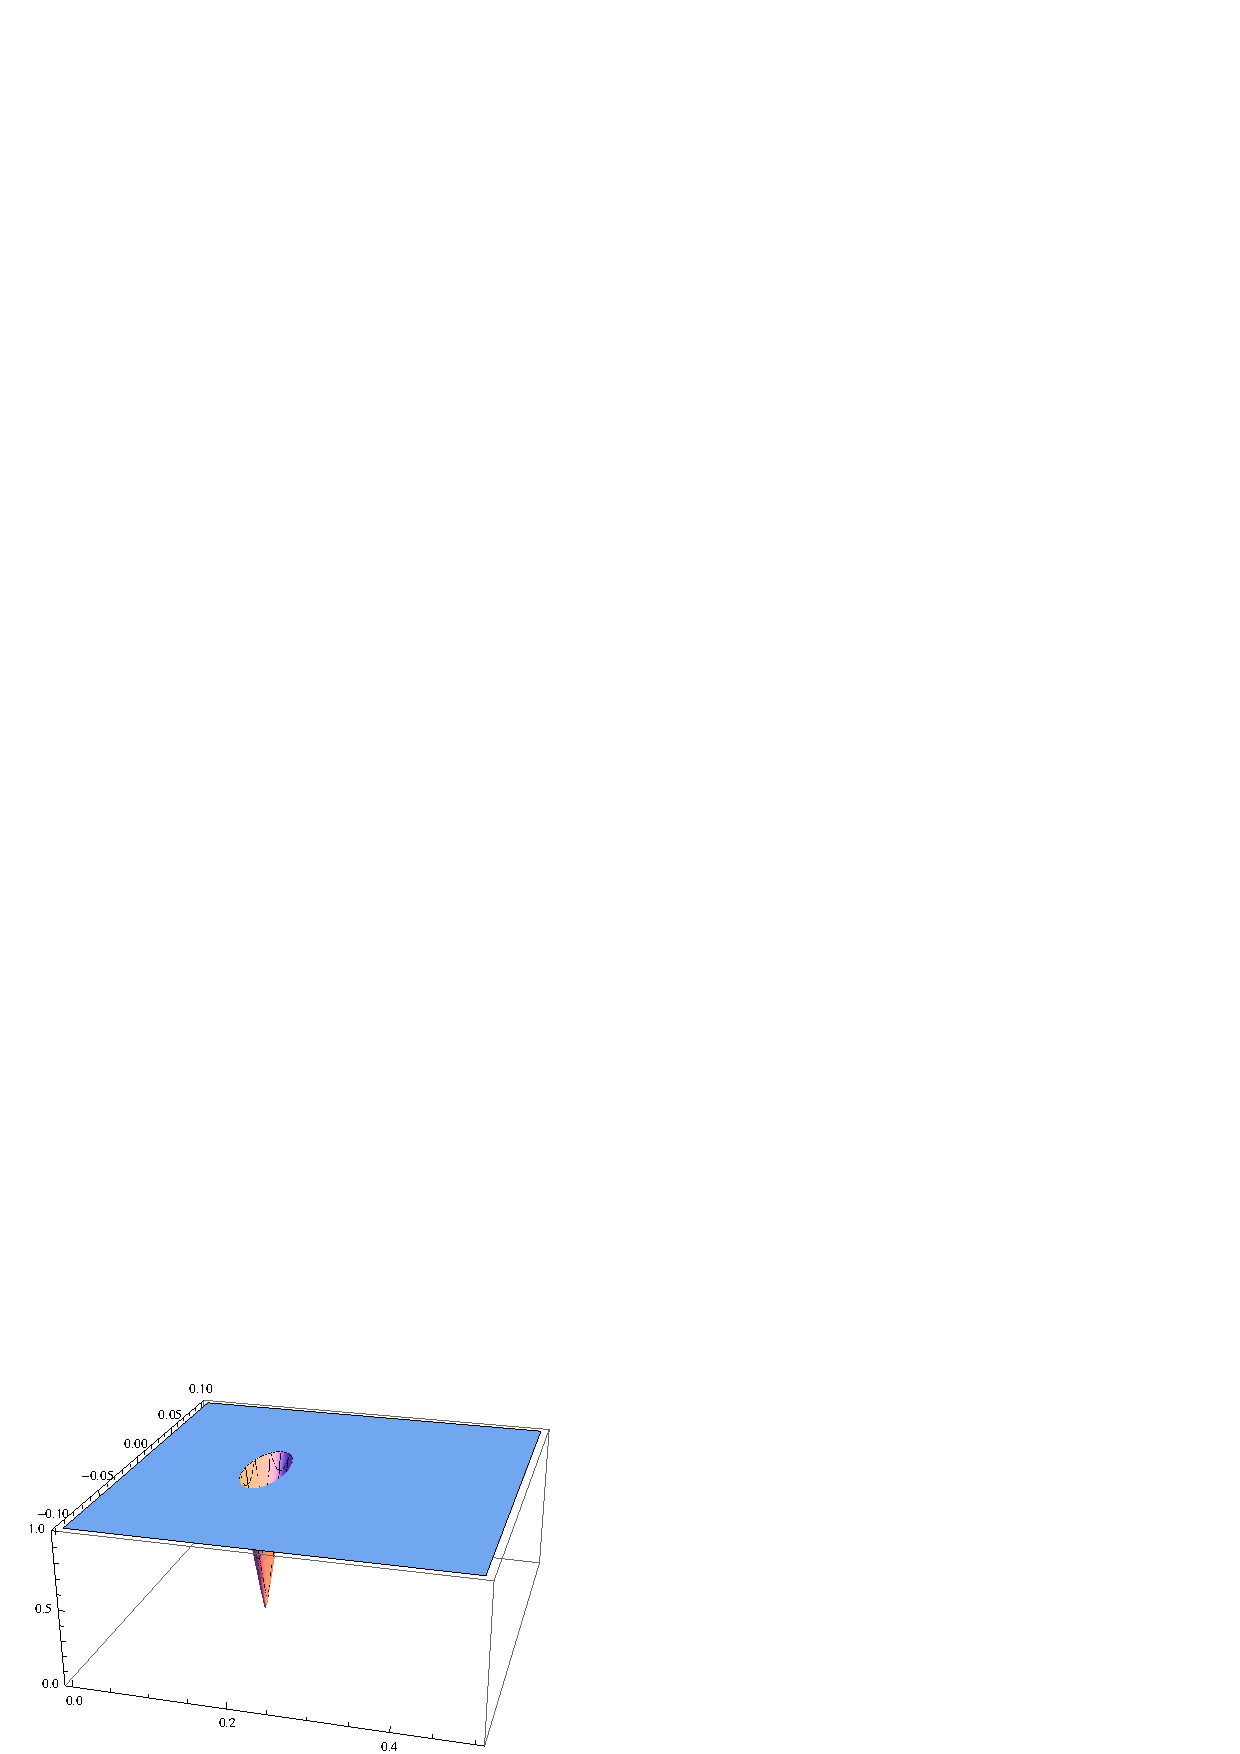
\includegraphics[width=.7\textwidth]{Est_ex2.png}
		\caption{$\left|O'_p\left(s_i(\gamma),\gamma\right)\right|$, $i=2,3$.}
		\label{estt}
	\end{minipage}
	%\end{minipage}
\end{figure}
%
%\begin{center}
%\begin{figure}[ht!]
%%\hspace{4cm}
%\includegraphics[width=.5\textwidth]{FamiliaTraub.eps}
%  \caption{Bifurcation diagram of fixed and critical points}\label{diagramabifurcacion}
%\end{figure}
%\end{center}

%\newpage

%%%%%%%%%%%%%%%%%%%%%%%%%%%%%%%%%%%%%%%%%%%%%%%%%%%%%%%%%%%
\section{El plano de parámetros}

Como hemos visto, el comportamiento dinámico del operador $O_p(z,\gamma)$ depende del valor del parámetro $\gamma$. El plano de parámetros asociado con un punto crítico libre de la familia (\ref{generalizacion}) es obtenido asociando cada punto del plano de parámetros con un valor complejo de $\gamma$, eso es, con un elemento de la familia (\ref{generalizacion}). Cada valor de $\gamma$ perteneciente a la misma componente conectada del plano de parámetros, da lugar a subconjuntos de métodos de la familia (\ref{generalizacion}) con un comportamiento dinámico similar. Así pues, es interesante encontrar áreas del plano de parámetros que sean lo más estables posible, ya que estos valores de $\gamma$ nos darán los mejores miembros de la familia, en términos de estabilidad numérica.

\begin{figure}[h!!!]
	\centering
	\subfloat[Plano de parámetros $P_1$]{\label{fig3:a}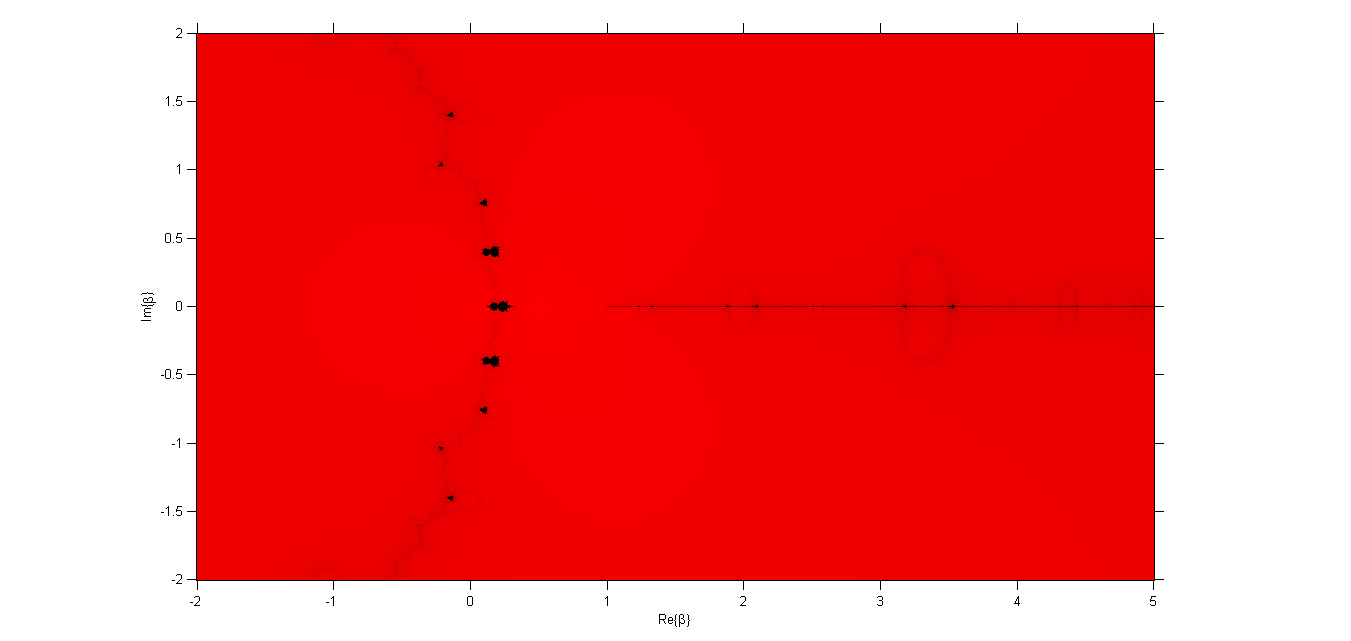
\includegraphics[width=.85\linewidth]{PlanoParametrico2_c1_2000pt_1000it_rojo.png}}\\
	\subfloat[Un detalle concreto]{\label{fig3:b}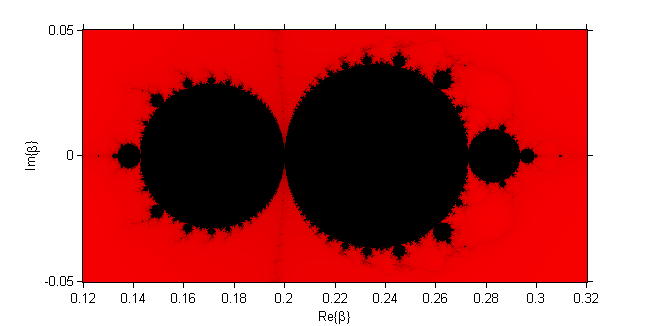
\includegraphics[width=0.4\textwidth]{PlanoParametrico_c1_2000pt_1000it_rojo.png}}
	\subfloat[Un detalle concreto]{\label{fig3:c}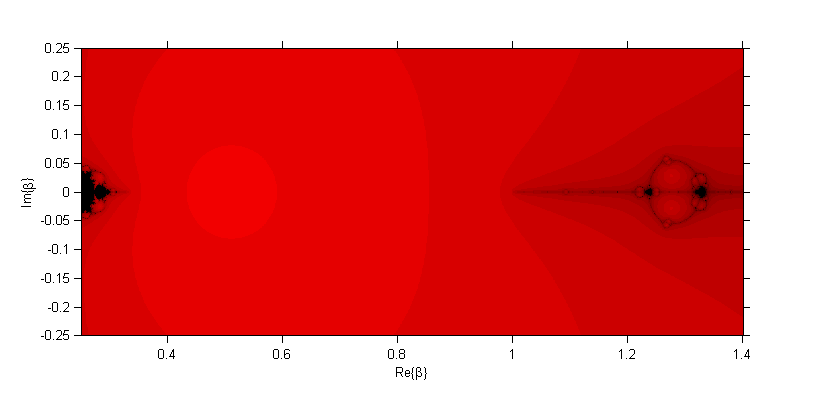
\includegraphics[width=0.42\textwidth]{PlanoParametrico3_c1_1000pt_200it_rojo.png}}
	\caption{Plano de parámetros $P_1$ y dos detalles concretos de éste}
	\label{planopar1}
\end{figure}

Dado que $cr_1(\gamma)=\frac{1}{cr_2(\gamma)}$, tenemos un sólo punto crítico libre independiente, por lo que también tenemos un sólo plano de parámetros, al que llamamos $P_1$. Cuando consideramos el punto crítico libre $z=cr_1(\gamma)$ como punto inicial del método iterativo de la familia (\ref{generalizacion}) asociado a cada valor complejo de $\gamma$, pintamos este punto del plano complejo en rojo si el método converge a alguna de las raíces (cero o infinito) y en negro en caso contrario. El color usado es más luminoso cuanto menor es el número de iteraciones requeridas para alcanzar la solución. El plano de parámetros que aparece en la Figura \ref{fig3:a} ha sido generado mediante el uso de ligeras modificaciones en las rutinas descritas en \cite{CCT}. Un mallado de $2000\times 2000$ puntos ha sido usado, 1000 ha sido el máximo número de iteraciones permitidas y $10^{-3}$ la tolerancia usada como criterio de parada. Observemos en dicha Figura \ref{fig3:a}  una gran estructura vertical que contiene (en el medio) el detalle que aparece en la Figura \ref{fig3:b}. Las otras regiones negras que aparecen en esta estructura son conjuntos de tipo Mandelbrot y se corresponden con distintos comportamientos periódicos.

%\begin{figure}[ht!]
%\begin{center}
%  \includegraphics[width=10cm]{planoparametrosfamiliaking2.eps}\\
%  \caption{Parameter space associated to $z=cr_i$, $i=1,2$}\label{planopar2}
%   \end{center}
%\end{figure}

Podemos observar (en la Figura \ref{fig3:b}) dos grandes discos negros en el centro de la figura: esta es la región donde los puntos fijos extraños $s_{2,3}(\gamma)$ (el disco de la izquierda) y $s_1(\gamma)$ (el disco de la derecha) son atractores o superatractores (ver Teorema \ref{teoestabilidad2}). 
%Furthermore, in Figure \ref{fig3:a}, we can observe a black cardioid joint to a black circle
%located around $\gamma=0.1\pm 0.4$, corresponding to orbits of
%period 2.

En la Figura \ref{fig3:b}, a la derecha del disco negro más grande vemos uno más pequeño, el cual ahora mostraremos que se corresponde a valores de $\gamma$ para los cuales también existen órbitas atractoras de periodo 2. Además, en la Figura \ref{fig3:c} se muestra la región cercana al cero, donde se hacen visibles ambas antenas. Observemos que, en estas antenas, aparecen algunos conjuntos de tipo Mandelbrot mostrando comportamientos periódicos.

Resumiendo, observamos que la mayor parte del plano complejo se corresponde a valores del plano de parámetros con comportamiento estable, mientras que algunos casos patológicos aparecen en regiones muy pequeñas.

%\begin{figure}[h!!!]
%    \centering
%    \includegraphics[width=.8\linewidth]{PlanoParametrico2_c1_1000pt_200it_rojo.eps}
%
%    \begin{minipage}[m]{0.5\linewidth}% \hspace{1cm}
%        \centering \includegraphics[width=.9\linewidth]{PlanoParametrico_c1_1000pt_200it_rojo.eps}
%    \end{minipage}
%    \begin{minipage}[m]{0.49\linewidth}% \hspace{1cm}
%        \centering 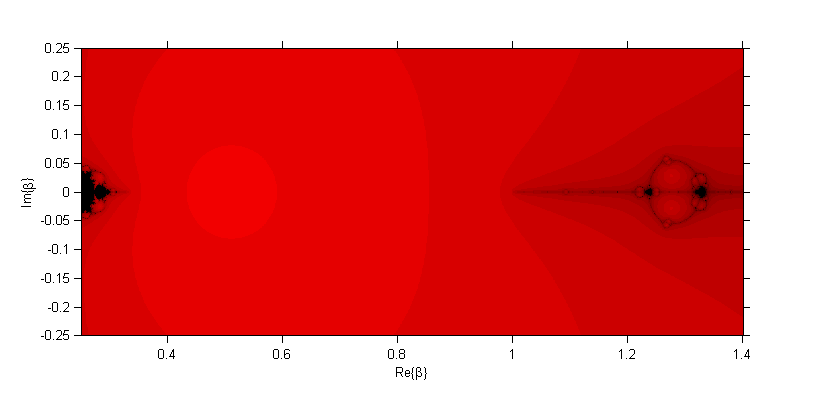
\includegraphics[width=1\linewidth]{PlanoParametrico3_c1_1000pt_200it_rojo.eps}
%    \end{minipage}
%
%    \caption{General view of the parameter plane $P_1$}\label{planopar1}
%\end{figure}


%%%%%%%%%%%%%%%%%%%%%%%%%%%%%%%%%%%%%%%%%%%%%%%%%%%%%%%%%%%
\section{Órbitas de periodo dos}

Con el objetivo de obtener la expresión analítica de los elementos de las órbitas periódicas de periodo 2, dependiendo de $\gamma$, calculamos $O_{p}(O_{p}(z,\gamma))$, que denotaremos como $O_{p}^2(z,\gamma)$,
{\small\begin{align*}
	&O_{p}^2(z,\gamma)=\frac{z^9 (\gamma  (z+2)-1)^3 \left(-\gamma  \left(z^3+4 z+1\right)+\gamma ^2 \left(z^4+2 z^3+4 z+2\right)+z\right)}{(\gamma +2 \gamma  z-z)^3 \left(z^3+\gamma ^2 \left(2 \left(z^4+2 z^3+z\right)+1\right)-\gamma  \left(z^4+4 z^3+z\right)\right)}.
	\end{align*}}

Los puntos periódicos de $O_{p}(z,\gamma)$ de periodo dos son las raíces de la ecuación $O_{p}^2(z,\gamma)=z$. Es decir, los puntos fijos anteriormente calculados y los puntos periódicos
\begin{equation*}
\begin{array}{ll}
pe_{\{1,2\}}(\gamma)=-\frac{\sqrt{5 \gamma ^2-2 \gamma +1}}{4 \gamma }\pm\frac{1}{2} \sqrt{\frac{(3 \gamma -1)^2}{2 \gamma ^2}-\frac{\gamma  \left(-\frac{(3 \gamma -1)^3}{\gamma ^3}+\frac{4 (3 \gamma -1)^2}{\gamma ^2}-\frac{8 (3 \gamma -1)}{\gamma }\right)}{2 \sqrt{5 \gamma ^2-2 \gamma +1}}-\frac{3 \gamma -1}{\gamma }-2}-\frac{3 \gamma -1}{4 \gamma },\\
%pe_2(\gamma)=-\frac{1}{4} \sqrt{4 \gamma +1}+\frac{1}{2} \sqrt{-\frac{12 (4-\gamma )-51}{2 \sqrt{4 \gamma +1}}+\gamma -\frac{3}{2}}-\frac{3}{4},\\
%pe_3(\gamma)=\frac{1}{4} \sqrt{4 \gamma +1}-\frac{1}{2} \sqrt{\frac{12 (4-\gamma )-51}{2 \sqrt{4 \gamma +1}}+\gamma -\frac{3}{2}}-\frac{3}{4},&
pe_{\{3,4\}}(\gamma)=\frac{\sqrt{5 \gamma ^2-2 \gamma +1}}{4 \gamma }\pm\frac{1}{2} \sqrt{\frac{(3 \gamma -1)^2}{2 \gamma ^2}+\frac{\gamma  \left(-\frac{(3 \gamma -1)^3}{\gamma ^3}+\frac{4 (3 \gamma -1)^2}{\gamma ^2}-\frac{8 (3 \gamma -1)}{\gamma }\right)}{2 \sqrt{5 \gamma ^2-2 \gamma +1}}-\frac{3 \gamma -1}{\gamma }-2}-\frac{3 \gamma -1}{4 \gamma },
\end{array}
\end{equation*}
y también las raíces del polinomio
\begin{align*}
	r(z)= & z^8 \gamma ^3+z^7 \left(3 \gamma ^3-2 \gamma ^2\right)+z^6 \left(2 \gamma ^3-3 \gamma ^2+\gamma \right)+z^5 \left(3 \gamma ^3-3 \gamma ^2+\gamma \right)\\\nonumber
	&+z^4 \left(9 \gamma ^3-11 \gamma ^2+5 \gamma -1\right)+z^3  \left(3 \gamma ^3-3 \gamma ^2+\gamma \right)\\\nonumber
	&+z^2 \left(2 \gamma ^3-3 \gamma ^2+\gamma \right)+z \left(3 \gamma ^3-2 \gamma ^2\right)+\gamma ^3,
\end{align*}
cuyas expresiones analíticas no hemos podido obtener.

En la Figura \ref{est1}, presentamos las regiones de estabilidad de
$pe_i(\gamma)$, $i=1,2$, y en la Figura \ref{est2}, presentamos las regiones de estabilidad de $pe_i(\gamma)$, $i=3,4$. Éstas representan el área compleja donde $|{O'_{\gamma}}^2(x)|<1$. En
la Figura \ref{estall} mostramos todas las regiones de estabilidad que pueden ser comparadas con el plano de parámetros de la Figura \ref{fig3:a}.

\begin{figure}[h!!!]
	\begin{minipage}[m]{0.49\linewidth}%
		\centering 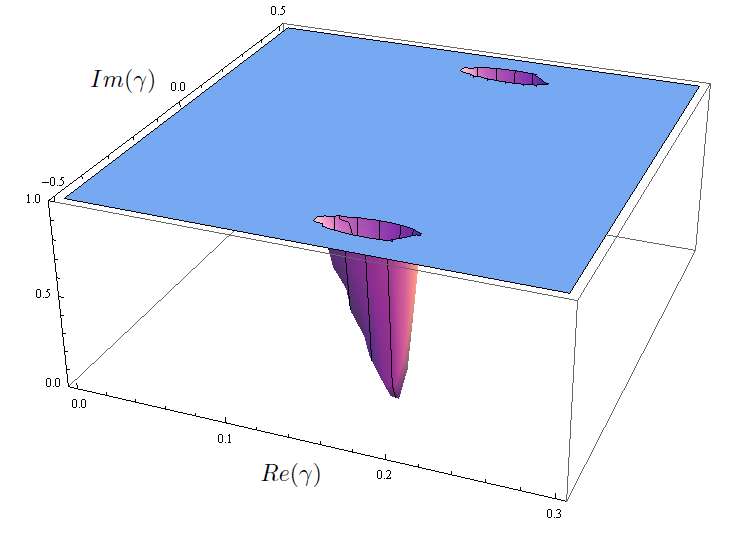
\includegraphics[width=.6\textwidth]{Est_pe12.png}
		\caption{$\left|{O'_{p}}^2\left(pe_i(\gamma),\gamma\right)\right|$, $i=1,2$}\label{est1}
	\end{minipage}
	\begin{minipage}[m]{0.49\linewidth}% \hspace{1cm}
		\centering 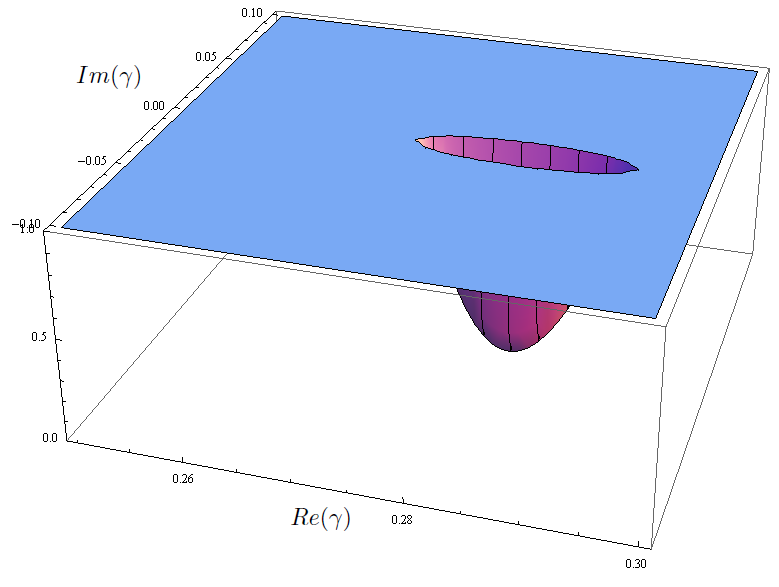
\includegraphics[width=.6\textwidth]{Est_pe23.png}
		\caption{$\left|{O'_{p}}^2\left(pe_i(\gamma),\gamma\right)\right|$, $i=3,4$}\label{est2}
	\end{minipage}
\end{figure}


\begin{figure}[h!!!]
	\centering
	%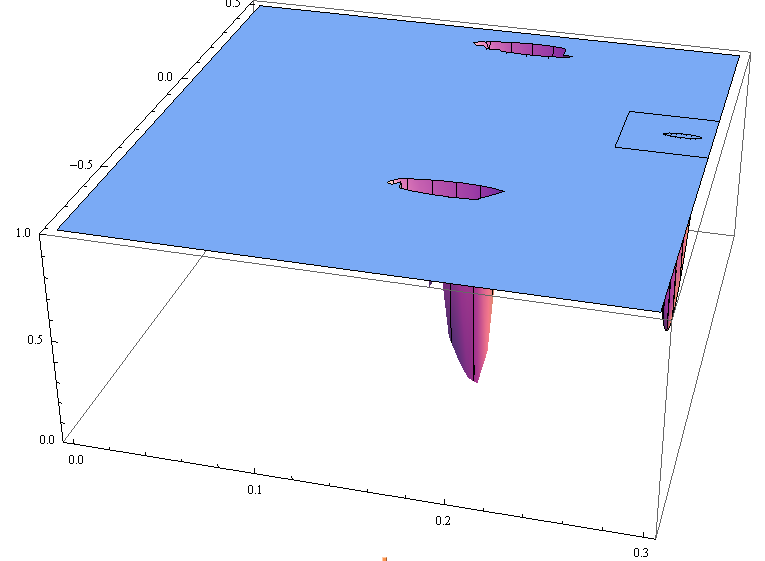
\includegraphics[width=0.35\textwidth]{Est_all.png}
	%    \hspace{1.5cm}
	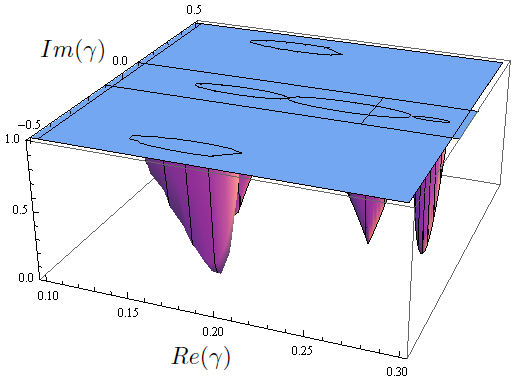
\includegraphics[width=0.5\textwidth]{Est_all2.png}
	\caption{Regiones de estabilidad (todas juntas)}\label{estall}
\end{figure}

Además, se puede comprobar que existen tres valores del parámetro $\gamma$ que hacen que las órbitas periódicas de periodo dos sean superatractoras, esto es, que se satisfaga ${O'_{p}}^2(z,\gamma)=0$. Estos valores son $\gamma= 0.19239 \pm
i0.40009$ y $\gamma=0.28187$, y pertenecen a dos cardioides negros de la gran estructura del plano de parámetros $P_1$, y al bulbo de la derecha del disco negro más grande de la Figura \ref{fig3:b}, respectivamente.

%%%%%%%%%%%%%%%%%%%%%%%%%%%%%%%%%%%%%%%%%%%%%%%%%%%%%%%%%%
\section{Planos dinámicos}

En esta sección se muestra, mediante planos dinámicos, el comportamiento cualitativo de algunos métodos particulares de la familia \eqref{generalizacion}. Estos elementos serán seleccionados a partir de las conclusiones obtenidas en el análisis del plano de parámetros de la familia. 

Como en el caso del plano de parámetros, estos planos dinámicos han sido generados mediante el uso de las rutinas que aparecen en \cite{CCT}. El plano dinámico asociado a un valor del parámetro $\gamma$, esto es, el correspondiente a un elemento de la familia \eqref{generalizacion}, es generado mediante el uso de cada punto del plano complejo como estimación inicial (hemos usado un mallado de $400\times 400$ puntos). Hemos pintado en azul los puntos cuyas órbitas convergen a infinito, en naranja los puntos que convergen al cero (con una tolerancia de $10^{-3}$), en verde los puntos cuya órbita converja a uno de los puntos fijos extraños (todos los puntos fijos aparecen marcados como una estrella blanca en las figuras) y en negro si alcanza el número máximo de 40 iteraciones sin converger a alguno de los puntos fijos.  

La mayor parte de las regiones del plano de parámetros $P_1$ corresponden a métodos iterativos con un buen comportamiento numérico, en términos de estabilidad y eficiencia. Se corresponden con los valores de $\gamma$ pintados en rojo. En las Figuras \ref{estable3}, \ref{estable4}, \ref{estable1} y \ref{estable2} mostramos distintos comportamientos estables correspondientes a diversos valores de $\gamma$ seleccionados en estas regiones rojas; en concreto usamos $\gamma=\frac{1}{2}$ (método de Homeier), $\gamma=-0.4$, $\gamma=0.4$ y $\gamma=-0.08$.

\begin{figure}[h!!!]
	\begin{minipage}[m]{0.5\linewidth}%
		\centering 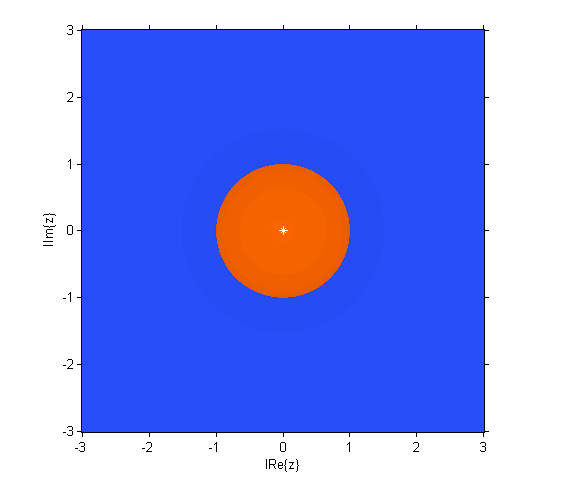
\includegraphics[width=\linewidth]{redpoint3.png}
		\caption{Plano dinámico asociado a $\gamma=0.5$}\label{estable3}
	\end{minipage}
	\begin{minipage}[m]{0.5\linewidth}% \hspace{1cm}
		\centering 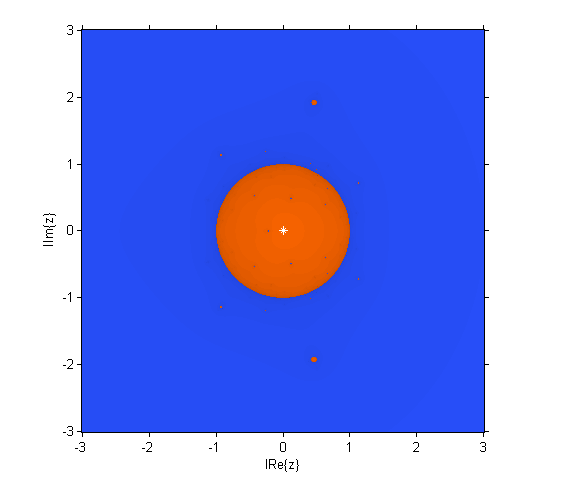
\includegraphics[width=\linewidth]{redpoint4.png}
		\caption{Plano dinámico asociado a $\gamma=-0.4$}\label{estable4}
	\end{minipage}
\end{figure}

\begin{figure}[h!!!]
	\begin{minipage}[m]{0.5\linewidth}%
		\centering 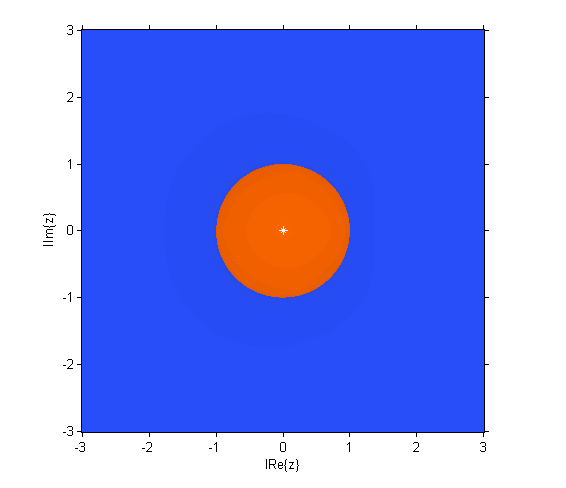
\includegraphics[width=\linewidth]{redpoint1.png}
		\caption{Plano dinámico asociado a $\gamma=0.4$}\label{estable1}
	\end{minipage}
	\begin{minipage}[m]{0.5\linewidth}% \hspace{1cm}
		\centering 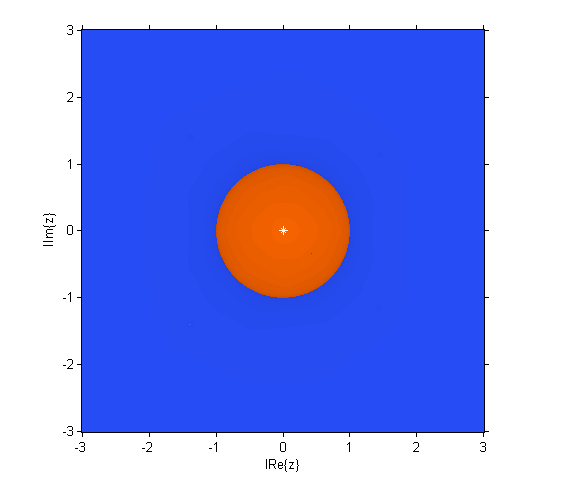
\includegraphics[width=\linewidth]{redpoint2.png}
		\caption{Plano dinámico asociado a $\gamma=-0.08$}\label{estable2}
	\end{minipage}
\end{figure}

Por otra parte, se encuentra comportamiento inestable cuando cogemos valores de $\gamma$ en las regiones negras del plano de parámetros $P_1$. En la Figura \ref{dospuntosfijos} se presenta el plano dinámico del método iterativo correspondiente a $\gamma=0.181$, mostrando la existencia de cuatro cuencas de atracción distintas, dos de ellas de los superatractores $0$ y $\infty$, y las otras dos correspondientes a los atractores $s_{2}(\gamma)$ y $s_{3}(\gamma)$. De forma análoga, en la Figura \ref{puntofijo1} vemos, además de las cuencas de atracción del $0$ y el $\infty$, aquella correspondiente al atractor $s_{1}(\gamma)$.

\begin{figure}[h!!!]
	\begin{minipage}[m]{0.5\linewidth}%
		\centering 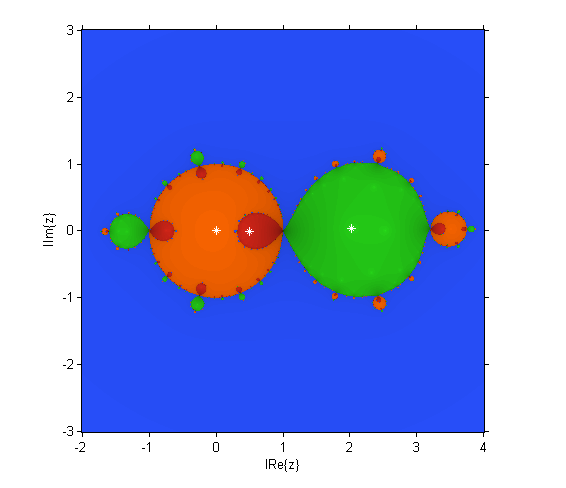
\includegraphics[width=\linewidth]{dospuntosfijos.png}
		\caption{Plano dinámico asociado a $\gamma=0.181$}\label{dospuntosfijos}
	\end{minipage}
	\begin{minipage}[m]{0.5\linewidth}% \hspace{1cm}
		\centering 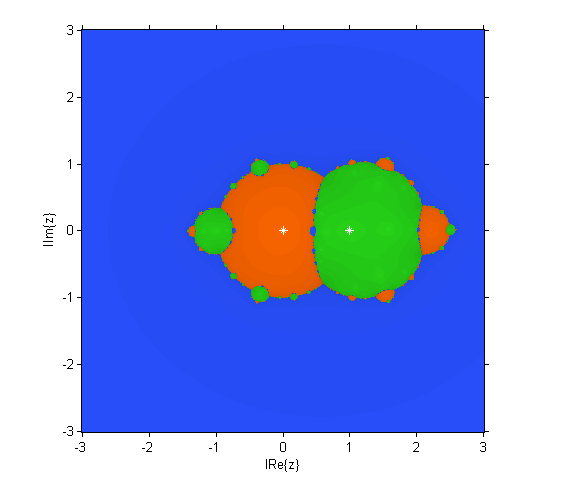
\includegraphics[width=\linewidth]{puntofijo1.png}
		\caption{Plano dinámico asociado a $\gamma=0.23$}\label{puntofijo1}
	\end{minipage}
\end{figure}

La Figura \ref{cardioide} corresponde al plano dinámico obtenido para $\gamma=0.1752+0.4i$, mostrando la existencia de tres cuencas de atracción distintas, dos de ellas de los superatractores $0$ y $\infty$, y la otra correspondiente a una órbita atractora de periodo 2.

\begin{figure}[h!!!]
	\begin{minipage}[m]{0.5\linewidth}%
		\centering 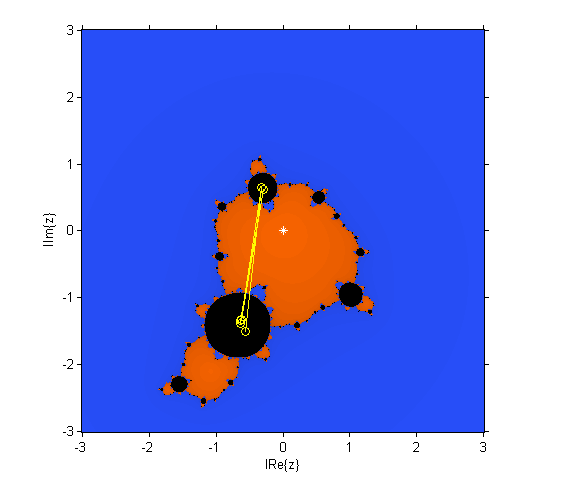
\includegraphics[width=\linewidth]{cardioide.png}
		\caption{Plano dinámico asociado a $\gamma=0.1752+0.4i$}\label{cardioide}
	\end{minipage}
	\begin{minipage}[m]{0.5\linewidth}% \hspace{1cm}
		\centering 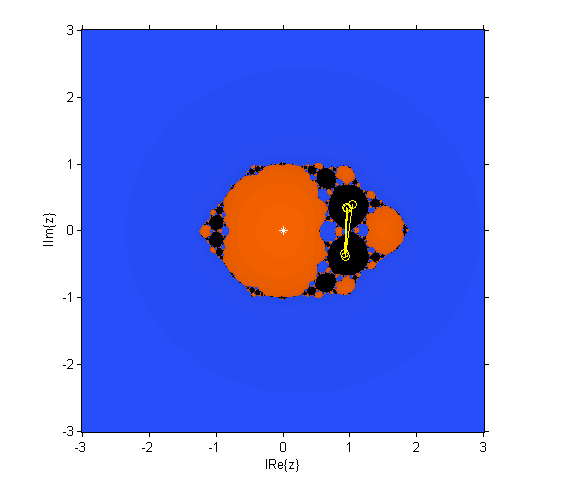
\includegraphics[width=\linewidth]{rightcircle.png}
		\caption{Plano dinámico asociado a $\gamma=0.283$}\label{rightcircle}
	\end{minipage}
\end{figure}

Otras regiones del plano de parámetros $P_1$ donde hay órbitas atractoras de periodo 2, son aquellas correspondientes a las Figuras \ref{rightcircle} y \ref{circulocardioide}. Nótese que en ésta última (Figura \ref{circulocardioide}) hay dos órbitas de periodo 2 distintas, con un punto crítico libre contenido en cada una de sus cuencas de atracción. Una órbita de periodo 4 es encontrada en el plano dinámico correspondiente a $\gamma=1.24$, como se muestra en la Figura \ref{4periodorbit}, que se corresponde a valores de $\gamma$ contenidos en uno de los conjuntos de Mandelbrot en la izquierda de la antena del plano de parámetros (ver Figura \ref{fig3:c}).

\begin{figure}[h!]
	\subfloat[]{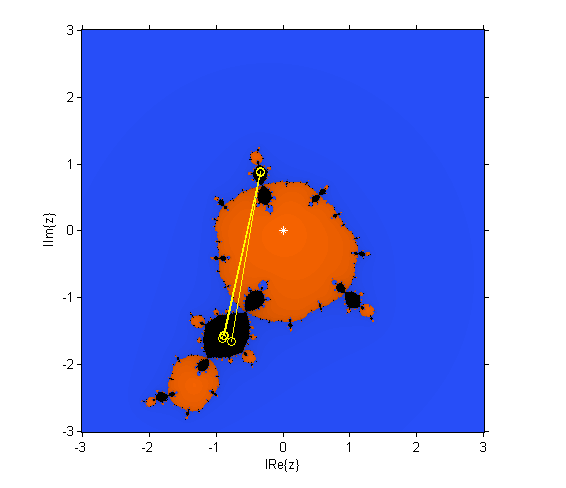
\includegraphics[width=0.50\textwidth]{circlecardioide1.png}}
	\subfloat[]{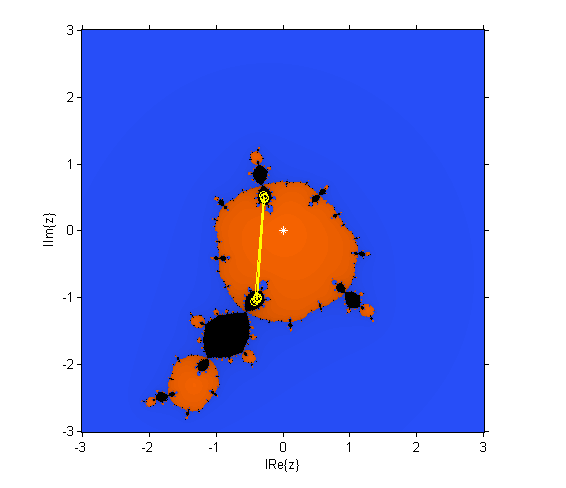
\includegraphics[width=0.50\textwidth]{circlecardioide2.png}}
	\caption{Planos dinámicos asociados a $\gamma=0.12+0.4i$}\label{circulocardioide}
\end{figure}


\begin{figure}[h!]
	\subfloat[$\gamma=1.24$]{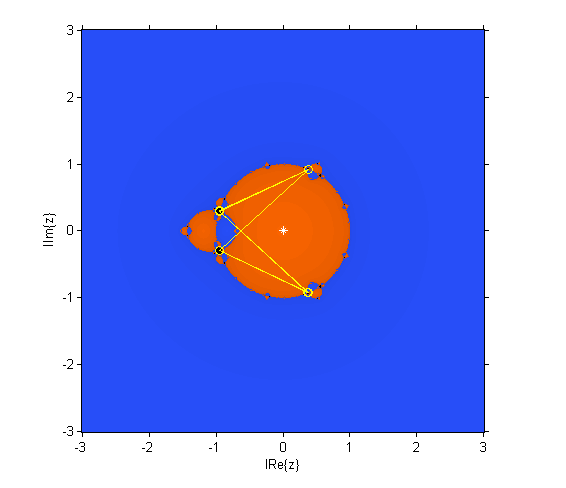
\includegraphics[width=0.50\textwidth]{4periodorbit.png}\label{4periodorbit}}
	\subfloat[$\gamma=0.31$]{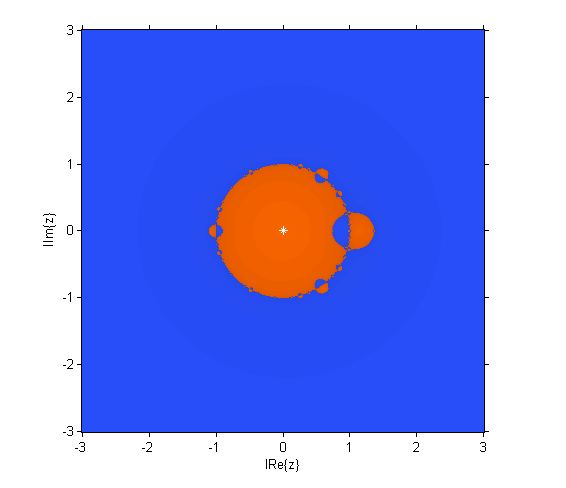
\includegraphics[width=0.50\textwidth]{antena.png}\label{antena}}
	\caption{Planos dinámicos para diferentes valores de $\gamma$.}
\end{figure}

Por último, el plano dinámico correspondiente a $\gamma=0.31$ se muestra en la Figura \ref{antena} con el objetivo de ver el comportamiento de la derecha de la antena en $P_1$; incluso este área muestra una muy buena estabilidad del método. 

\section{Conclusiones}

El comportamiento dinámico de la familia \eqref{generalizacion} sobre polinomios cuadráticos es muy rico. Analizando los planos de parámetros, se ha mostrado que algunos valores del parámetro $\gamma$, eso es, miembros de la familia, pueden no converger a las raíces. La existencia de órbitas periódicas de periodo 2 ha sido mostrada, y su expresión analítica ha sido obtenida en términos del parámetro $\gamma$. Sin embargo, es importante recalcar que algunos de las áreas inestables encontradas en $P_1$ se corresponden con valores complejos del parámetro $\gamma$, los cuales son muy raramente usados, y en consecuencia la gran mayoría del plano de parámetros se corresponde con métodos iterativos con un muy buen comportamiento numérico.